\begin{figure}[H]
    \centering
    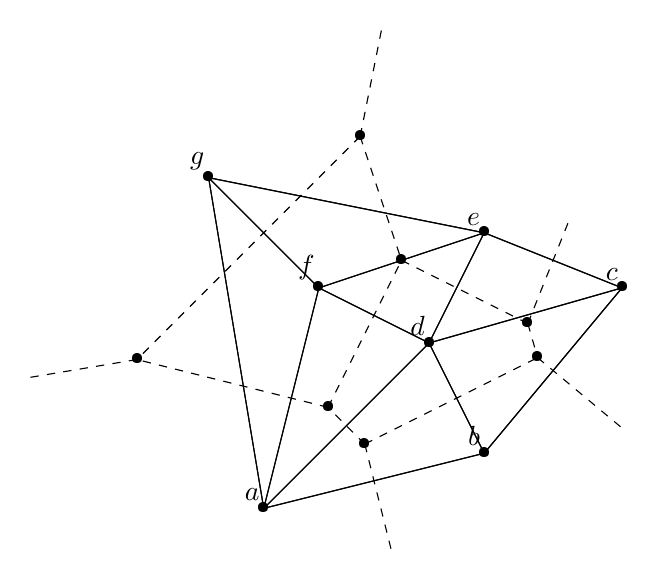
\begin{tikzpicture}[scale=0.7]
        \node[label={[label distance = -3mm]160:$a$}] at (-3.0, 0) {\textbullet};
        \node[label={[label distance = -3mm]160:$b$}] at (1, 1) {\textbullet};
        \node[label={[label distance = -3mm]160:$c$}] at (3.5, 4.0) {\textbullet};
        \node[label={[label distance = -3mm]160:$d$}] at (0, 3) {\textbullet};
        \node[label={[label distance = -3mm]160:$e$}] at (1, 5) {\textbullet};
        \node[label={[label distance = -3mm]160:$f$}] at (-2.0, 4) {\textbullet};
        \node[label={[label distance = -3mm]160:$g$}] at (-4, 6) {\textbullet};
        \draw (-3.0, 0) -- (1, 1);
        \draw (1, 1) -- (-3.0, 0);
        \draw (0, 3) -- (1, 1);
        \draw (1, 1) -- (0, 3);
        \draw (3.5, 4.0) -- (1, 1);
        \draw (1, 1) -- (3.5, 4.0);
        \draw (-3.0, 0) -- (0, 3);
        \draw (0, 3) -- (-3.0, 0);
        \draw (0, 3) -- (3.5, 4.0);
        \draw (3.5, 4.0) -- (0, 3);
        \draw (-2.0, 4) -- (0, 3);
        \draw (0, 3) -- (-2.0, 4);
        \draw (1, 5) -- (0, 3);
        \draw (0, 3) -- (1, 5);
        \draw (1, 5) -- (3.5, 4.0);
        \draw (3.5, 4.0) -- (1, 5);
        \draw (-3.0, 0) -- (-2.0, 4);
        \draw (-2.0, 4) -- (-3.0, 0);
        \draw (-2.0, 4) -- (1, 5);
        \draw (1, 5) -- (-2.0, 4);
        \draw (-3.0, 0) -- (-4, 6);
        \draw (-4, 6) -- (-3.0, 0);
        \draw (-4, 6) -- (-2.0, 4);
        \draw (-2.0, 4) -- (-4, 6);
        \draw (-4, 6) -- (1, 5);
        \draw (1, 5) -- (-4, 6);

        \node (abd) at (-1.1666666666666667, 1.1666666666666667) {\textbullet}; % a-b-d
        \draw[dashed] (-1.1666666666666667, 1.1666666666666667) -- (-1.8333333333333333, 1.8333333333333333); %abd--afd
        \draw[dashed] (-1.1666666666666667, 1.1666666666666667) -- (1.96875, 2.734375); %abd--dbc
% a -- b
        \draw[dashed] (-1.1666666666666667, 1.1666666666666667) -- (-0.6815954165940006, -0.773618333623997);
        \node (afd) at (-1.8333333333333333, 1.8333333333333333) {\textbullet}; % a-f-d
        \draw[dashed] (-1.8333333333333333, 1.8333333333333333) -- (-0.5, 4.5); %afd--fed
        \draw[dashed] (-1.8333333333333333, 1.8333333333333333) -- (-5.3, 2.7); %afd--afg
        \node (dbc) at (1.96875, 2.734375) {\textbullet}; % d-b-c
% b -- c
        \draw[dashed] (1.96875, 2.734375) -- (3.505192559194752, 1.4540062006710404);
        \node (afg) at (-5.3, 2.7) {\textbullet}; % a-f-g
% g -- a
        \draw[dashed] (-5.3, 2.7) -- (-7.272787847664287, 2.3712020253892856);
        \node (fge) at (-1.25, 6.75) {\textbullet}; % f-g-e
        \draw[dashed] (-1.25, 6.75) -- (-0.5, 4.5); %fge--fed
        \draw[dashed] (-1.25, 6.75) -- (-5.3, 2.7); %fge--afg
% e -- g
        \draw[dashed] (-1.25, 6.75) -- (-0.8577677297236319, 8.71116135138184);
        \node (fed) at (-0.5, 4.5) {\textbullet}; % f-e-d
        \node (edc) at (1.7916666666666667, 3.3541666666666665) {\textbullet}; % e-d-c
        \draw[dashed] (1.7916666666666667, 3.3541666666666665) -- (-0.5, 4.5); %edc--fed
        \draw[dashed] (1.7916666666666667, 3.3541666666666665) -- (1.96875, 2.734375); %edc--dbc
% c -- e
        \draw[dashed] (1.7916666666666667, 3.3541666666666665) -- (2.534448019374874, 5.211120048437185);
    \end{tikzpicture}
    \caption[Exemplo da dualidade entre Delaunay e Voronoi]{Exemplo da dualidade entre a triangulação de Delaunay e o Diagrama de Voronoi. Os segmentos tracejados são as arestas do diagrama. Os segmentos traçados são as arestas da triangulação.}\label{fig:delaunay:dual}
\end{figure}
